\def\year{2016}\relax
%File: formatting-instruction.tex
\documentclass[letterpaper]{article}
\usepackage{aaai16}
\usepackage{times}
\usepackage{helvet}
\usepackage{courier}
\usepackage{graphicx}
\usepackage{subcaption}
\usepackage{tikz}
\usepackage{enumitem}
\usepackage{xspace}

\def\checkmark{\tikz\fill[scale=0.4](0,.35) -- (.25,0) -- (1,.7) -- (.25,.15) -- cycle;} 
\newcommand{\eg}{\textit{e.g.,}\@\xspace}
\newcommand{\ie}{\textit{i.e.,}\@\xspace}

\makeatletter
\newcommand{\etc}{%
    \@ifnextchar{.}%
        {\textit{etc}}%
        {\textit{etc.}\@\xspace}%
}

\frenchspacing
\setlength{\pdfpagewidth}{8.5in}
\setlength{\pdfpageheight}{11in}

\pdfinfo{
/Title (CRQA: Crowd-powered Real-time Automated Question Answering System)
/Author (Denis Savenkov, Eugene Agichtein)}
\setcounter{secnumdepth}{0}

\begin{document}
% The file aaai.sty is the style file for AAAI Press 
% proceedings, working notes, and technical reports.
%
\title{CRQA: Crowd-powered Real-time Automated Question Answering System}
\author{
	Denis Savenkov\\
	Emory University\\
	\texttt{dsavenk@emory.edu}
\And
	Eugene Agichtein\\
	Emory University\\
	\texttt{eugene@mathcs.emory.edu}
}

\maketitle
\begin{abstract}
Modern search engines have made dramatic progress in answering questions about facts, such as those that might be retrieved or directly inferred from a knowledge base.
However, many other real user questions are more complex, such as requests for opinions, explanations, instructions or advice for a particular situation, and are still largely beyond the competence of the computer systems.
As conversational agents become more popular, QA systems are increasingly expected to handle such complex questions, and to do so in (nearly) real-time, as the searcher is unlikely to wait longer than a minute or two for an answer.
One way to overcome some of the challenges in complex question answering is crowdsourcing.
We explore two ways crowdsourcing can assist a question answering system that operates in (near) real time: by providing answer {\em validation}, which could be used to filter or re-rank the candidate answers, and by {\em creating} the answer candidates directly.
In this paper we present CRQA, a crowd-powered, near real-time automatic question answering system for complex informational tasks, that incorporates a crowdsourcing module for augmenting and validating the candidate answers.
The crowd input, obtained in real-time, is integrated into CRQA via a learning-to-rank model, to select the final system answer.
Our large-scale experiments, performed on a live stream of real users questions, show that even within a one minute time limit, CRQA can produce answers of high quality.
The returned answers are judged to be significantly better compared to the automatic system alone, and even are often preferred to answers posted days later in the original community question answering site.
Our findings can be useful for developing hybrid human-computer systems for automatic question answering and conversational agents.
\end{abstract}

\section{Introduction}
\label{sec:introduction}

It has long been a dream to communicate with a computer as one might with another human being using natural language speech and text.
We are now coming closer to this dream, as natural language interfaces become increasingly popular.
Our phones are already reasonably good at recognizing speech, and personal assistants, such as Apple Siri, Google Now, Microsoft Cortana, Amazon Alexa, \etc, help us with everyday tasks and answer some of our questions.
Chat bots are arguably considered ``the next big thing'', and a number of startups developing this kind of technology has emerged in Silicon Valley and around the world\footnote{http://time.com/4194063/chatbots-facebook-messenger-kik-wechat/}.

Question answering is one of the major components of such personal assistants.
Existing techniques already allow users to get direct answers to their factoid questions.
However, there is still a large number of more complex questions, such as advice or accepted general opinions, for which users have to dig into the ``10 blue links'' and extract or synthesize answers from information buried within the retrieved documents.
To cater to these informational needs, community question answering (CQA) sites emerged, such as Yahoo! Answers and Stack Exchange.
These sites provide a popular way to connect information seekers with answerers.
Unfortunately, it can take minutes or hours, and sometimes days, for the community to respond, and some questions are left unanswered altogether. 

To facilitate research on this challenge, a series of TREC LiveQA evaluation campaigns\footnote{http://www.trec-liveqa.org} was introduced in 2015, where automatic systems attempt to answer real user questions within a 1 minute period.
This task was successful, with the winning system able to automatically return a reasonable answer to more than half of the submitted questions, as assessed for TREC by the trained judges from NIST.
Nevertheless, many questions were not answered well by any of the participating systems~\cite{overviewliveqa15}.

In this work we explore two ways \textit{crowdsourcing} can be used to help an automatic system answer complex user questions.
The main challenge is how to adapt existing ``batch-mode'' crowdsourcing platforms such as Amazon Mechanical Turk to real-time settings, \eg to produce an answer within a minute.
More specifically, our research questions can be stated as:
\textbf{RQ1}. Can crowdsourcing be used to improve the performance of a near real-time automatic question answering system?
\textbf{RQ2}. What kind of contributions from crowd workers can help improve automatic question answering and what is the relative impact of different types of feedback to the overall question answering performance?
\textbf{RQ3}. What are the trade-offs in performance, cost, and scalability of using crowdsourcing for real-time question answering?

To explore these research questions, we introduce our CRQA system, which stands for Crowd-powered Real-time Question Answering.
CRQA integrates a crowdsourcing module into an automatic question answering system within an overall learning-to-rank framework for selecting answers to complex questions.
We report extensive experiments of stress-testing the CRQA system, by participating in the TREC LiveQA 2016 evaluation challenge.
Specifically, the contributions of this paper are threefold:
\begin{enumerate}
	\item CRQA, a novel hybrid near real-time question answering system, that uses crowd workers to rate and augment automatically generated candidate answers, developed to empirically explore the research questions above.
	\item Large scale experiments using CRQA to answer real user questions in a live TREC LiveQA 2016 challenge setting, addressing \textbf{RQ1}.
	\item Extensive analysis of the system performance, focusing on the contributions of crowd input to the performance of the overall system, to explore \textbf{RQ2} and \textbf{RQ3}.
\end{enumerate}

The results and findings of this work can be useful to guide future research on hybrid human-computer question answering, and automatic intelligent assistant systems.

\section{System design}
\label{sec:system}

Before diving into the architecture of our Crowd-powered Real-time Question Answering (CRQA) system, we will describe the setup of the TREC LiveQA shared task, which affected some of the system design choices.
In 2015 and 2016 versions of the task participants of the challenge developed a live question answering system, that responded to user questions, which were sampled from the live stream of Yahoo! Answers community question answering website.
Each input question consisted of a short question title, body and category (Figure~\ref{fig:ya_question}).
A QA system had to provide an answer of 1000 characters or less within a 1 minute period using any available data source.
A reader can refer to \cite{overviewliveqa15} for more details on TREC LiveQA 2015 results and analysis.

\begin{figure*}[h!t]
	\centering
	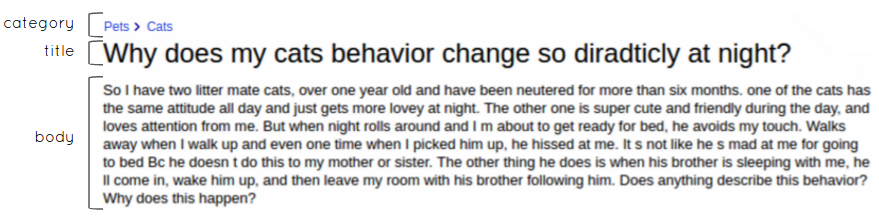
\includegraphics[width=0.75\textwidth]{img/ya_question}
	\caption{Example of the question from Yahoo! Answers community question answering platform}
	\label{fig:ya_question}
\end{figure*}

\begin{figure*}[h!t]
	\centering
	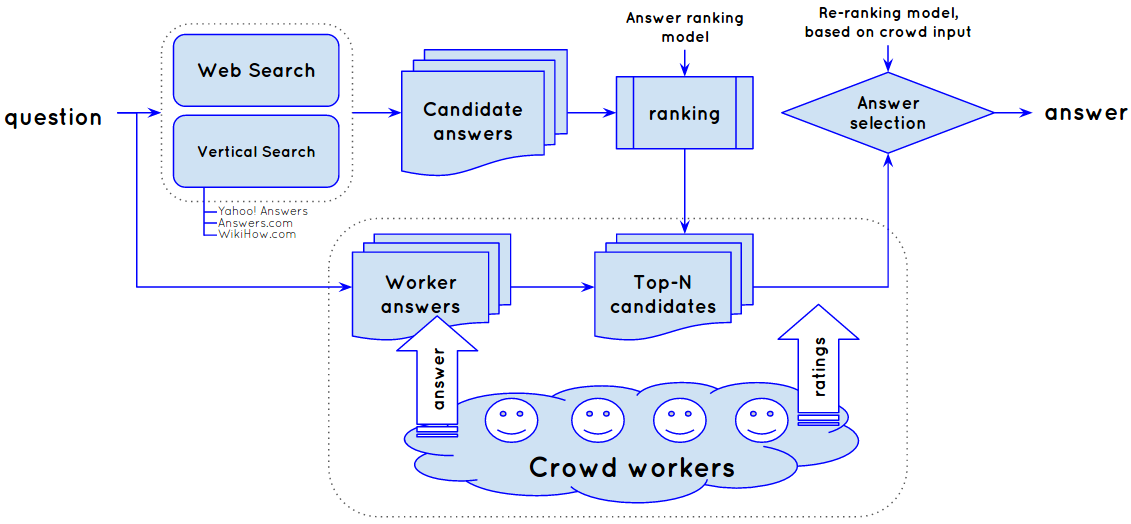
\includegraphics[width=0.8\textwidth]{img/system}
	\caption{The architecture of our Crowd-powered Real-time Question Answering system, that uses crowdsourcing to augment a list of automatically extracted candidate answers and to rate their quality}
	\label{fig:system}
\end{figure*}

Our CRQA system represents a hybrid system, that includes an automatic question answering and crowdsourcing modules.
The high level architecture is presented in Figure~\ref{fig:system}.
The automatic part of the CRQA system follows an Information Retrieval (IR) approach to question answering, and generates a set of candidate answer passages from multiple data sources.
After candidates are generated, they are ranked by a trained model, and, in the fully automatic mode, the top candidate could be returned as the answer.
The crowdsourcing module is designed to overcome two of the most common problems of the automatic QA approaches: lack of good candidate answers and ranking errors~\cite{moldovan2003performance,savenkov_trecliveqa15}.
More particularly, CRQA asks crowd workers to provide answers to questions if they can, and additionally rate the quality of candidate answers.
These contributions are then used to re-rank the candidates and return the top scoring answer.
The next two sections describe the architectures of the automatic and crowdsourcing modules of our system.

\subsection{Automatic question answering module}
\label{sec:system:auto}

When CRQA receives a question, it generates a set of search queries to retrieve a set of relevant documents and extract candidate answer passages.
Search queries are generated using the following strategies:
\begin{itemize}
\item Question title, which most often captures the gist of the question
\item Two longest question sentences (detected by the presence of the question word at the beginning or question mark at the end of a sentence) from the title and body of the question. In some cases the real user question is hidden inside the body, while the title just provides the overall topic of the question.
\item Concatenation of the question word, verbs and top-5 terms from the question title by inverse document frequency\footnote{IDF of terms are estimated using Google N-gram corpus: https://catalog.ldc.upenn.edu/LDC2006T13}. This strategy targets over-specific questions (\eg Figure~\ref{fig:ya_question}), which often retrieve few if any search results.
\end{itemize}

To retrieve a set of potentially relevant documents and extract candidate answer passages, CRQA relies on multiple different generic and CQA document collections.
Previous research has shown that many of the user information needs are repeated, and reusing answers to previously posted similar questions is an effective strategy for answering new questions~\cite{carmel2000eresponder,shtok2012learning}.
Therefore, CRQA uses multiple different CQA data sources, namely Yahoo! Answers, Answers.com and WikiHow.com, which potentially contain a diverse set of questions.
To retrieve similar questions we use the built-in search interfaces of the corresponding websites.
CRQA extracts top-10 similar questions and the corresponding answers, posted by the community, and adds them to the pool of candidate answers.
However, quite often it is hard to find a similar question in an archive, and many of the information needs are unique.
Therefore, we integrate web search\footnote{https://datamarket.azure.com/dataset/bing/searchweb}, which our system queries to retrieve candidate answers from regular web documents.
We retrieve top-10 relevant web documents and extract paragraphs of text from their main content, as detected by a method based on \cite{Kohlschutter_2010}.

In addition to the candidate answers themselves, CRQA extracts certain meta-data, that helps to estimate the relevance of a passage to the current question.
For regular web page paragraphs, it is useful to know the topic of the page (\eg its title) and the context (such as text that immediately precedes the paragraph in the document).
For CQA answers, our system stores the text of the corresponding question title, body and category.
For convenience, we will refer to this question title and web page title as \textit{``answer topic''}, while the body of the retrieved question and the preceding text block for web candidates as \textit{``answer context''}.
Next, for each candidate answer we compute a set of features, described in Table \ref{table:features}.

\begin{table}[ht]
\centering
\begin{tabular}{| p{7.8cm} |}
\hline
\textbf{Answer statistics} \\
\hline
--- Length in chars, words and sentences \\
--- Average number of words per sentence \\
--- Fraction of non-alphanumeric characters  \\
--- Number of question marks \\
--- Number of verbs  \\
\hline
\textbf{Answer source} \\
\hline
--- Binary feature for each of the search verticals: Web, Yahoo! Answers, Answers.com, WikiHow.com \\
\hline
\textbf{N-gram matches}\\
\hline
--- Cosine similarities using uni-, bi- and tri-gram representations of the question title and/or body, and answer text, topic or context\\
--- The lengths of longest spans of matched terms between question title and/or body, and answer text, topic or context\\
\hline
\textbf{Information Retrieval score}\\
\hline
--- BM25 scores between question title and/or body, and answer text, topic or context\\ 
\hline
\end{tabular}
\caption{The list of candidate answer ranking features used by the automatic module of our CRQA system}
\label{table:features}
\end{table}

At the final stage of the module, answers are ranked by their predicted quality.
We chose to use the LambdaMART learning to rank algorithm, which was proven to be very successful for various ranking problems~\cite{burges2010ranknet}.
This model was trained using the RankLib library\footnote{https://sourceforge.net/p/lemur/wiki/RankLib/} on the data from last year TREC LiveQA task\footnote{https://sites.google.com/site/trecliveqa2016/liveqa-qrels-2015}, which includes 1087 questions with answers provided by the participants, each of which was rated on a scale from 1(bad) to 4(excellent) by professional NIST assessors.
In a fully automatic setup the top ranked candidate is returned as the final answer to the question.

\subsection{Crowdsourcing module}
\label{sec:system:crowd}

Unfortunately, fully automatic QA systems still struggle with many difficult questions~\cite{overviewliveqa15}, therefore we decided to explore crowdsourcing as one of the ways to help the system to deal with these questions.
Instead of immediately returning the answers, CRQA sends questions and top-7 ranked candidates to crowd workers and waits for the responses.
We chose to give 7 answers based on the average number of rated answers in our preliminary studies~\cite{savenkov_crowdsourcing2016a}.
Since in TREC LiveQA systems had only 60 seconds to answer each question, we start a timer when a question arrives, and the system waits to receive all worker contributions until the timer reaches 50 seconds to leave some time to generate the final answer.
To help resolve the cases when the automatic QA module was not able to generate good candidates, we ask workers to provide their own answers, if possible.
Additionally, workers are expected to rate the provided answers, which should help to improve the ranking.
Figure~\ref{fig:crowd_ui} presents the user interface of our crowdsourcing module.

\begin{figure*}[h!t]
	\centering
	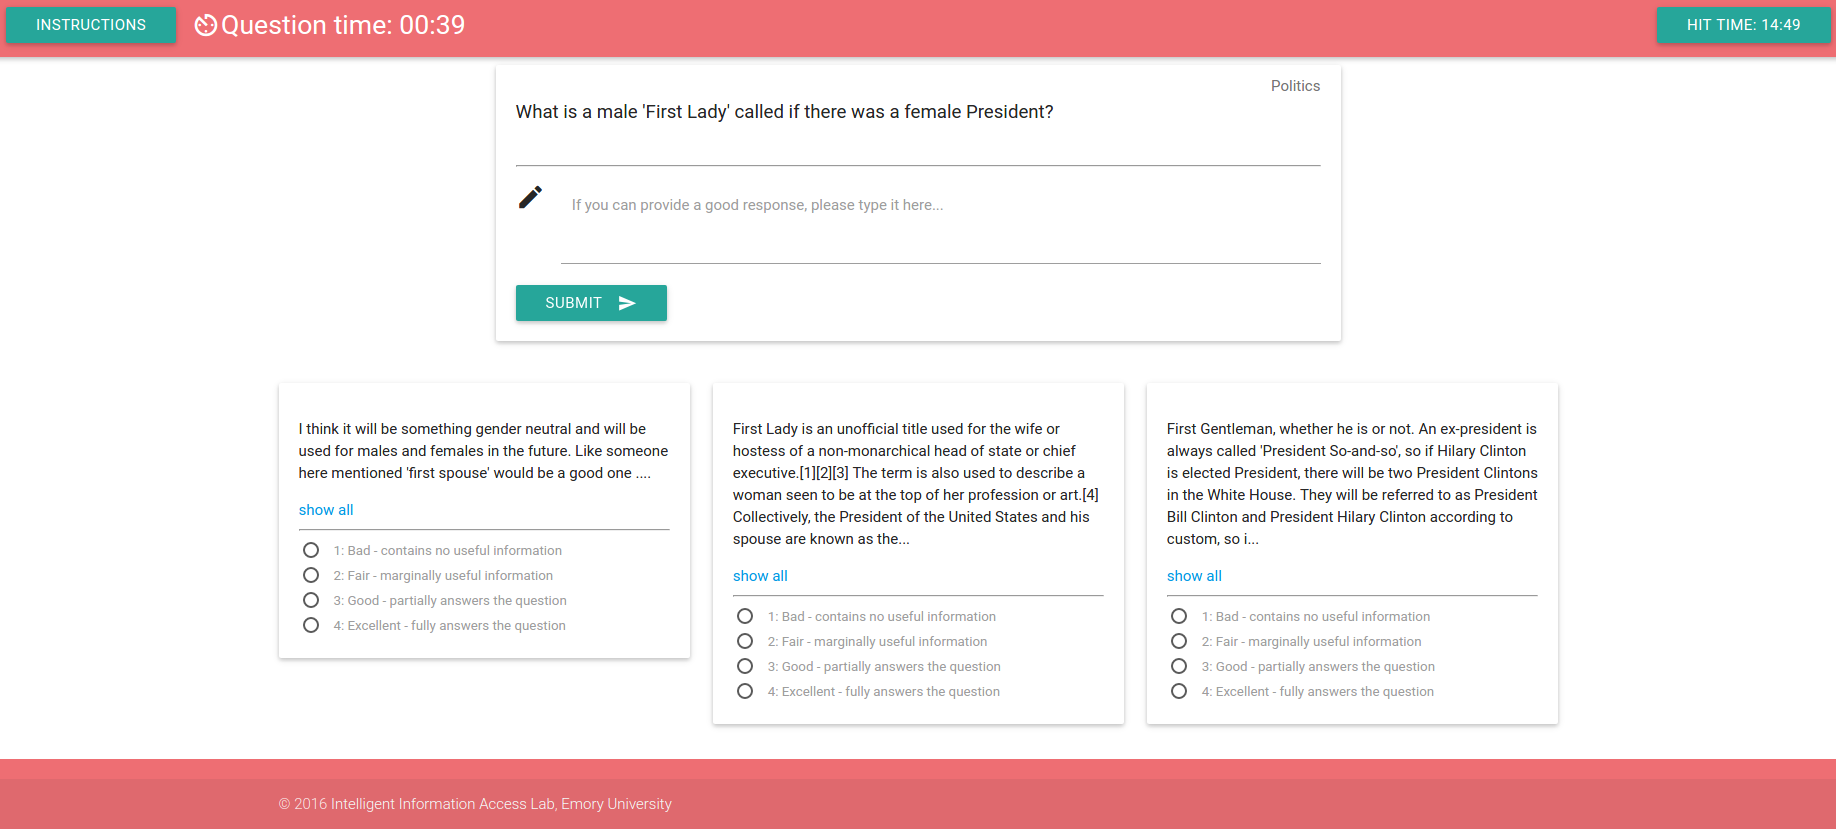
\includegraphics[width=0.9\textwidth]{img/crowd_ui}
	\caption{User Interface for workers in our Crowd-Powered Question Answering system}
	\label{fig:crowd_ui}
\end{figure*}

The overall algorithm for obtaining crowd input for real-time question answering is the following:
\begin{enumerate}
\item When a system receives a question, it is posted to workers, who have 50 seconds to provide their input
\item Workers are asked to write an answer if they can provide one (optional)
\item Otherwise they need to wait for answer candidates to appear
\item When a system is done generating and ranking candidates, it posts top-7 answers for rating (which usually happens $\sim$ 35 seconds before the question expires)
\item Workers receive a list of answers and rate them until the timer expires. Answers, provided by the workers, are also rated, except by their authors. Each answer is rated on a scale from 1 to 4, using the official TREC LiveQA rating scale:
	\begin{itemize}[noitemsep,topsep=0pt]
    \item 1 -- Bad: contains no useful information
    \item 2 -- Fair: marginally useful information
    \item 3 -- Good: partially answers the question
    \item 4 -- Excellent: fully answers the question
    \end{itemize}
\item The interface displays 3 answers at a time, when an answer gets rated, it disappears and its place is taken by another answer from the pool. The interface displays only the first 300 characters of the answer, which was experimentally shown to be enough on average to make a good judgment.
Full answer can be revealed upon clicking the ``show all'' link.
\item When the question expires, it disappears, and workers wait for the next question
\end{enumerate}

To hire the workers we used Amazon Mechanical Turk platform\footnote{http://mturk.com}.
Since the challenge was to run the system ``live'' over the period of 24 hours, we adapted the retainer model~\cite{bernstein2011crowds,bigham2010vizwiz}, \ie workers were paid to stay on our interface and complete the tasks for 15 minutes.
Specifically, to obtain an even distribution of workers over the 24-hour period of the TREC LiveQA shared task, we posted 10 tasks every 15 minutes.
Since not all assignments were accepted right away, the number of workers for each question varied and could be greater than 10.
When a worker first gets to our crowdsourcing interface, she is shown task instructions (Table \ref{table:crowd_instructions}) and asked to wait for the questions to arrive.
The workers were paid \$1.00 for a 15 minutes task, no matter how many questions they received.

We should note, that the setup of TREC LiveQA shared task was very favorable for the retainer crowdsourcing model, as the questions were arriving almost every minute uniformly over 24 hour period, which diminishes the waiting and worker idleness problems~\cite{Lasecki:2013:CCC:2501988.2502057}.
An interesting challenge, that we leave for future work, is how to adjust such a crowd-powered QA system to varying questions volume, while optimizing the costs.
One idea is to allocate crowdsourcing resources to the incoming questions proportionally to the expected effect, \ie order the questions by the expected performance of the automatically generated answer.
There are also certain techniques to optimize the costs of the retainer model~\cite{bernstein2012analytic}.
In addition, it is also possible to reduce the latency associated with hiring new workers on crowdsourcing platforms on demand, \eg using quikTurkIt approach from ~\cite{bigham2010vizwiz}.

\begin{table}[ht]
\centering
\begin{tabular}{| p{7.8cm} |}
\hline
\textbf{Instructions} \\
\hline
1. This HIT will last exactly 15 minutes\\
2. Your HIT will only be submitted after these 15 minutes\\
3. In this period of time you will receive some questions, that came from real users on the Internet\\
4. Each question has a time limit after which it will disappear and you will need to want for the next one\\
5. If you know the answer to the question, please type it in the corresponding box\\
6. At some point several candidate answers will appear at the bottom of the page\\
7. Please rate them on a scale from 1 (bad) to 4 (excellent)\\
8. Do not close the browser or reload the page as this will reset your assignment.\\
\hline
\end{tabular}
\caption{Crowdsourcing task instructions, displayed to the user when she first gets to the task}
\label{table:crowd_instructions}
\end{table}

\subsection{Answer re-ranking and selection}
\label{sec:system:reranking}

The last stage in CRQA is answer re-ranking, which aggregates all the information received from the crowdsourcing and produces the final answer to the question.
The input of the re-ranking module is a set of candidate answers with quality ratings provided by the crowd workers.
During the TREC LiveQA 2016 run we used a simple heuristic model, which ordered the answers by the average rating, and returned either the top candidate, if its average score was $\geq 2.5$, or the longest worker contributed answer.
After the challenge was over, we collected all the questions and answers, that were shown to the crowd workers.
The quality of each candidate answer was judged using traditional batch-mode crowdsourcing on the above mentioned scale from 1 (bad) to 4 (excellent).
Then, on a subset of the questions along with worker contributions, we trained a new model to re-rank the answers given all available crowdsourcing information.
The rest of the questions from TREC LiveQA 2016 run were used to evaluate the quality of the model.
This time, for convenience, we used Gradient Boosting Regression Trees~\cite{friedman2002stochastic} from scikit-learn Python package, and trained a regression model to predict the quality of the answer candidates.
The features, used for answer re-ranking are listed in Table \ref{table:reranking_features}.

\begin{table}[ht]
\centering
\begin{tabular}{| p{7.8cm} |}
\hline
\textbf{Answer-based} \\
\hline
--- The length of the answer \\
--- Source of the answer (Crowd, Web, Yahoo! Answers, Answers.com or WikiHow.com)\\
--- Original rank of the candidate answer or -1 for answers provided by the crowd workers\\
\hline
\textbf{Worker ratings} \\
\hline
--- Number of ratings provided\\
--- Minimum, maximum, median and average ratings\\
\hline
\end{tabular}
\caption{The list of features used for answer re-ranking based on crowdsourcing input}
\label{table:reranking_features}
\end{table}

\section{Experiments}
\label{sec:experiments}

\subsection{Experimental Setup: TREC LiveQA}

The experimental evaluation of our CRQA system was done on data from the official run of TREC LiveQA 2016 shared task, which happened on May 31, 2016.
All participating systems were running for 24 hours and received questions sampled from the live (real-time) stream of questions, posted to Yahoo! Answers.
In total, each system received 1,088 questions, and responses were recorded by the organizers.
Overall statistics are provided in Table \ref{table:task_stats}.
As we can see, on average, workers were able to provide at least one answer to each question, and 6 ratings for each answer.

\begin{table}[ht]
\centering
\begin{tabular}{| p{6.7cm} | c | }
\hline
Name & Value \\
\hline
Number of questions received & 1088 \\
Number of completed 15 min assignments & 889 \\
Avg number of questions per assignment & 11.44 \\
Total cost per question & \$0.81 \\
Avg number of answers provided by workers & 1.25 \\
Avg number of ratings per answer & 6.25 \\
\hline
\end{tabular}
\caption{Aggregate statistics of CRQA crowdsourcing tasks on TREC LiveQA 2016}
\label{table:task_stats}
\end{table}

\subsection{Answer Quality Evaluation}
\label{sec:experiments:answer-quality-evaluation}

We collected all the questions along with system candidates from the official TREC LiveQA 2016 run.
In addition, on June 2, two days after the TREC LiveQA challenge has completed, we crawled community answers for all task questions.
To obtain the quality labels for these answers and answer candidates, that were shown to crowd workers during the task, we used traditional (batch-mode) crowdsourcing.
All the answers were randomly shuffled and rated on a scale from 1 (bad) to 4 (excellent) by workers hired on Amazon Mechanical Turk\footnote{There was no time limit for rating this time}.
Existing research demonstrated, that such crowdsourced labels correlates well with the official ratings, provided by the professional NIST assessors~\cite{savenkov_crowdsourcing2016a}.
Each answer was labeled by 3 different workers, and we averaged the scores to get the final quality labels for the candidates.
As mentioned previously, we split the questions multiple times randomly into the training set to build a re-ranking model, and used the other split to evaluate the quality of the model.

\subsubsection{Methods compared.}
We compared CRQA system against several baselines:
\begin{itemize}
\item \textit{Automatic QA}: fully automatic QA system
\item \textit{CRQA}: automatic QA system with the crowdsourcing module and trained re-ranking model
\item \textit{Re-ranking by score}: a simplified version of CRQA re-ranking model, which selects the answer with the highest average ratings, provided by the crowd workers during the task.
\item \textit{Yahoo Answers}: traditional, non-real-time community question answering site (Yahoo! Answers), from which the challenge question originated.
The answers were collected two days after the challenge, thus allowing the Yahoo Answers community extra two days to collect the answers.
\end{itemize}

\subsubsection{Metrics.}
To evaluate the methods we used the metrics proposed by the organizers of the LiveQA task:
\begin{itemize}
\item \textbf{avg-score}: average score over all questions (missing answers receive a score of 0)
\item \textbf{avg-prec}: average score over all answered questions
\item \textbf{succ@i+}: the fraction of answers with score i or greater (i=2..4)
\item \textbf{prec@i+}: the number of answers with score i or greater (i=2..4) divided by the number of answered questions\footnote{Since for each answer we averaged 3 ratings by different workers, the number of answers with the average score of 4 is low}
\end{itemize}

\begin{table*}[ht]
\centering
\begin{tabular}{| p{3.5cm} | c | c | c | c | c | c | c | c |}
\hline
Method & avg-score & avg-prec & succ@2+ & succ@3+ & succ@4+ & prec@2+ & prec@3+ & prec@4+ \\
\hline
Automatic QA & 2.321 & 2.357 & 0.697 & 0.297 & 0.026 & 0.708 & 0.302 & 0.026 \\
Re-ranking by score & 2.416 & 2.421 & 0.745 & 0.319 & 0.031 & 0.747 & 0.320 & 0.031 \\
Yahoo! Answers & 2.229 & 2.503 & 0.656 & 0.375 & \textbf{0.045} & 0.737 & \textbf{0.421} & \textbf{0.050} \\
CRQA (ratings + ans.) & \textbf{2.550} & \textbf{2.556} & \textbf{0.799} & \textbf{0.402} & 0.034 & \textbf{0.800} & 0.402 & 0.034 \\
\hspace{5mm}worker ratings only & 2.432 & 2.470 & 0.750 & 0.348 & 0.030 & 0.762 & 0.354 & 0.031 \\
\hspace{5mm}worker answers only & 2.459 & 2.463 & 0.759 & 0.354 & 0.029 & 0.760 & 0.355 & 0.029 \\
\hline
\end{tabular}
\caption{Evaluation of the baselines and system answers quality based on the ratings of answers obtained via crowdsourcing. The scores are averaged over 100 different 50:50 splits of 1088 questions into the training and test set. The differences between average score and precision of CRQA and the original ranking are significant at p-value $<$ 0.01}
\label{table:performance}
\end{table*}

Table~\ref{table:performance} summarizes the performance of the baselines and our system.
As we can see, the average score and precision of answers generated by CRQA system is higher than the baseline ranking and even community answers on the Yahoo! Answers platform.
However, community answers have higher percentage of \textit{``4 (excellent)''} scores.
Figure~\ref{fig:score_histogram} shows the distribution of scores for the original system ranking, our crowdsourcing system and Yahoo! Answers.
Two peaks on the distribution of scores from Yahoo! Answers community suggest, that there are essentially two kinds of responses: non-useful (\eg spam) or excellent that fully answers the question.
In addition, around 20\% of the questions did not get any answer from the community.
Automatically generated answers, on the contrary, are rarely empty, but on average provide only marginally relevant information, which often does not answer the questions, and therefore rated \textit{``2 (fair)''}.
The introduction of the crowdsourcing module allowed CRQA to cover couple percents of the questions, for which the automatic system was not able to generate any candidates, as well as select better candidates when it was possible using crowd ratings.

\begin{figure}[h]
	\centering
	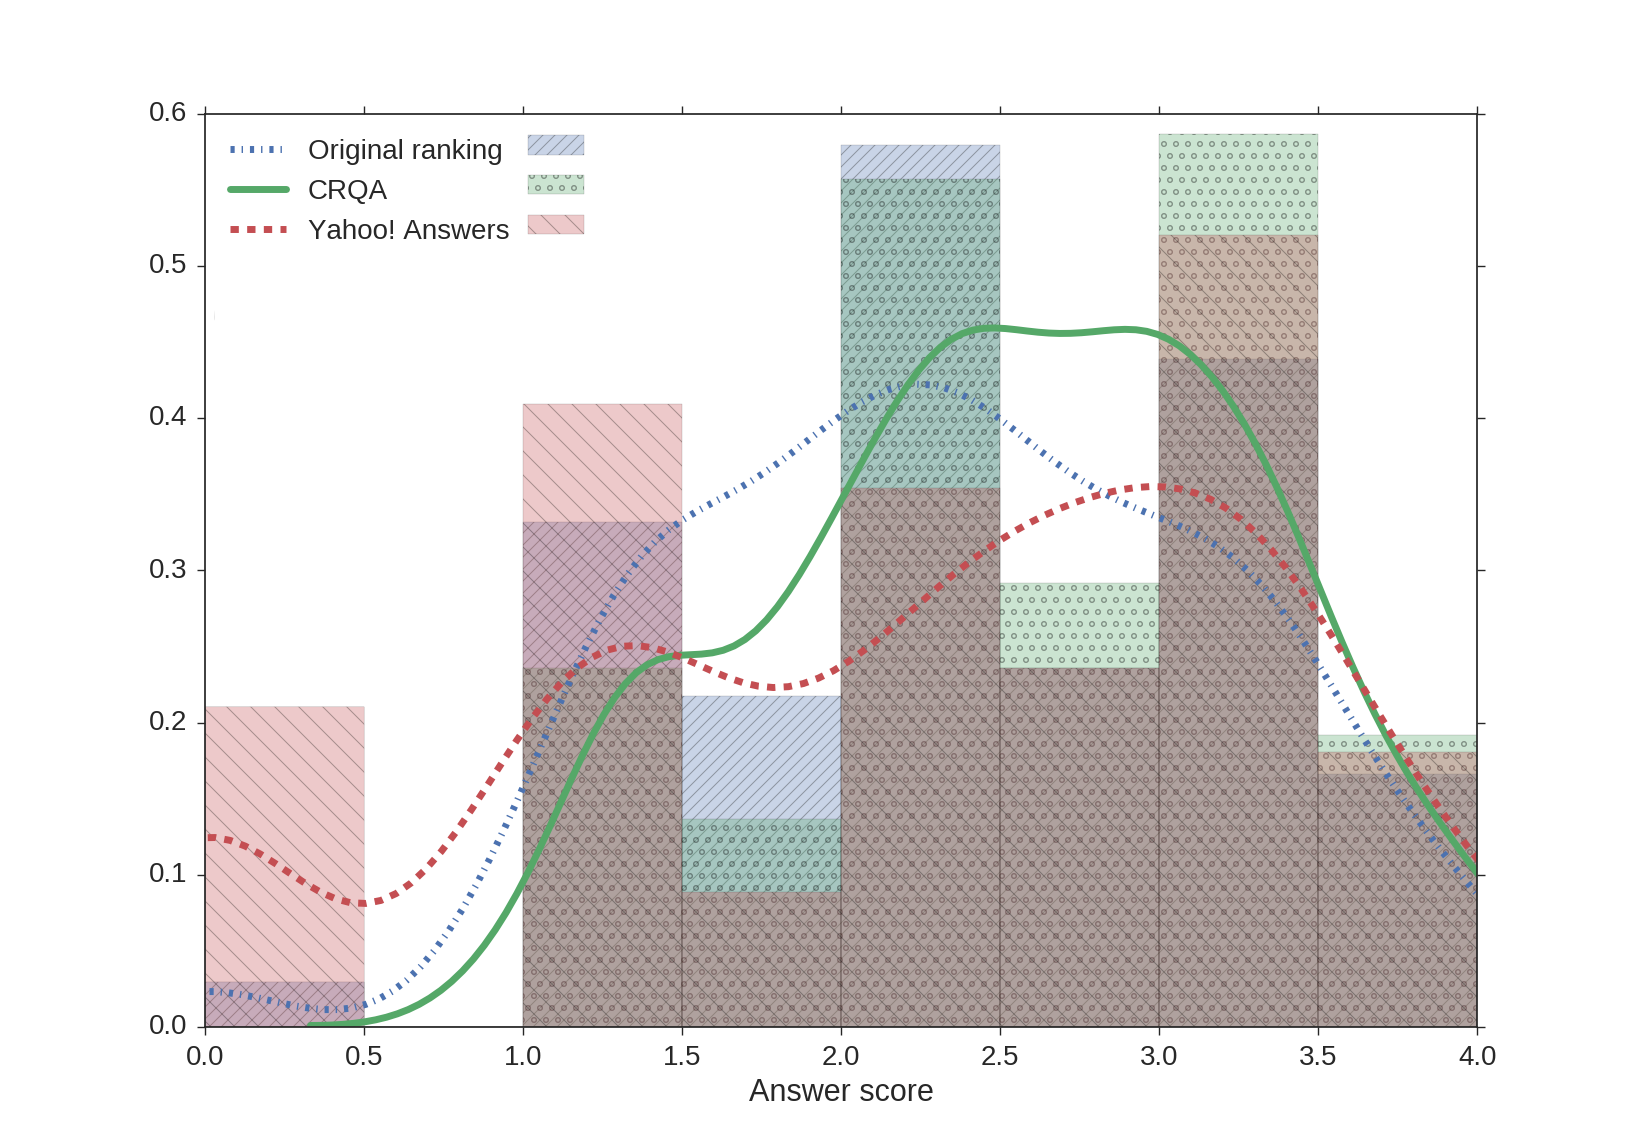
\includegraphics[width=0.46\textwidth]{img/score_hist}
	\caption{Histogram and kernel density estimation of answer scores for original candidate ranking, CRQA model re-ranking and Yahoo! Answers answers}
	\label{fig:score_histogram}
\end{figure}

% Can remove this sentence
Therefore, we can conclude, that crowdsourcing can effectively help the automatic QA system to improve the performance of question answering, by providing worker generated answers and rating existing candidates.
To get some insights into when crowdsourcing is more and less effective, we looked into the quality of the generated answers across different Yahoo! Answers categories.
Overall, CRQA improves upon the baseline fully automatic QA system across all the categories.
However, the absolute value of the average quality gain is different, \eg crowdsourcing had the biggest impact on the quality for the ``Travel'' category, which was one of the hardest for the fully automatic system~\cite{savenkov_trecliveqa15}.
On the other hand, for ``Arts \& Humanities'', ``Pets'' and ``Home \& Garden'' categories crowdsourcing was less efficient (but still improved the quality).
One of the reasons is that questions from these categories often require certain expertise or prior experience, which makes it harder for crowd workers to contribute.
To study this hypothesis we further sampled questions with lowest and highest differences in answer quality between the automatic system and CRQA.
Many of the questions, where crowdsourcing actually hurt the performance required some special knowledge, \eg ``\textit{Can someone help answer questions about scapholunate ligament surgery rehabilitation?}'' or ``\textit{What was pol pot's vision of an agrarian society? }''.
Examples, when crowdsourcing helped the most, include cases of automatic system failures, \eg no answer candidates or candidate, that only repeat the question and was ranked first by the system.

To summarize, our Crowd-powered Real-time Question Answering system substantially improves the quality compared to the baseline fully automatic system, and generated answers are often even preferred to responses posted by CQA community.

\section{Analysis and Discussion}
\label{sec:analysis}

In this section we will analyze some of the results of our experiments and discuss their implications.

\subsection{Worker answers vs ratings}
\label{sec:analysis:answers_vs_ratings}

First, let's look at the contribution of additional answers and ratings provided by the workers.
These two types of contributions are complimentary to each other and attempt to solve different problems.
Table~\ref{table:performance} shows the performance of our question answering system using each of these types of feedback independently.
The results demonstrate that both answers and ratings have positive effect on the performance.
Even with limited time, workers were able to reliably rate candidate answers, which helped the system to select a better final answer and improve the model precision.
However, this method does not help the system in cases, when it was not able to generate any good candidates in the first place, therefore using ratings only has lower average answer score than using worker generated answers.
By asking the crowd to provide a response if they can answer the question, CRQA covers this gap, which is important as in a real scenario even a fair answer would probably be better for the user than no answer at all.
Of course, given limited time and the fact that a random worker might not possess an expertise required, such answers do not always perfectly answer the question.
Table~\ref{table:answer_examples} gives some examples of worker generated answers with low and high quality scores.

To summarize, ratings of answer candidates and worker generated answers both have similar positive effect on the performance of our question answering system.
What is more important, the contributions are independent and therefore it is beneficial to use both of them in the final system.

\begin{table*}[ht]
\centering
\begin{tabular}{| p{10.2cm} | p{5cm} | c |}
\hline
Question & Answer & Score \\
\hline
 Is Gotu Kola a good herb for mental health? How long does it take to work?? & yes & 1.66\\
 \hline
Can I write any number on line number 5 of a W2?  would like to set up my W2 were I get the most out of my paycheck and not have to pay taxes at the end of the year... & W2 & 1.33\\
 \hline
I need help with my mum? Something traumatic happened to me about 4 years ago i randomly asked my mother why when I lived with you in your home country a man that was our neighbour used to call me his daughter and the younger kids that lived there called me there cousins and one boy called me his sister? & yes & 1.0\\
\hline
\hline
 Is it bad not wanting to visit your family? & It's nt bad. Just be honest with them. They may be upset but they should understand & 3.0 \\
 \hline
Any health concerns with whey protein? So I workout 3-5 days a week and i drink a whey protein isolate after each workout. Since I workout almost everyday, is it ok for me to just drink a shake everyday?.. & As long as you use it as directed, there should not be any major problems.  You may want to consult your doctor just in case, but I would not be too concerned. & 3.0\\
\hline
Foot pain unable to walk? Hi so today woke with some pain, I'm able to put weight on my heel with no problem or pain.  But  the area between my heel and toes hurts really bad when I try to go with the motion of taking a step. Its not swollen and I do not remember hurting it at all & Possible gout in your foot, also possible you may have strained it during the previous day. & 3.0\\
\hline
What is a good remedy/medicine for stomach aches? Specifically ones caused by stress or anxiety? & Chamomile tea should help & 3.66\\
\hline
\end{tabular}
\caption{Examples of answers provided by the crowd workers and their average quality scores}
\label{table:answer_examples}
\end{table*}

\subsection{Selection of answer candidate for rating}
\label{sec:analysis:order}

Predicting the quality of answers and ranking them to select the best is quite challenging for automatic question answering~\cite{surdeanu2011learning}.
External feedback, such as noisy answer ratings, obtained from the crowd workers, provides valuable information, which, as our results demonstrate, can help a QA system to better re-rank the answers.
However, the capacity of crowdsourcing for answer ratings are obviously limited, as systems often are dealing with hundreds and thousands of answer candidates for a given question.
In this work, we made a choice to rate only top-7 answers according the automatic system ranking.
This decision was made based on the average number of ratings workers could provide in the allotted time.
However, the order in which the answers are shown can also have a strong effect on the system performance, because the answers are typically rated one by one in the order they are displayed on the screen.
To study the effect of the answer presentation order on the final answer quality, our system implemented two different strategies, which were selected at random for each question and each worker.
The first strategy ordered the answers according to their predicted relevance score, and the other shuffled the answers randomly.
The later strategy provides a uniform coverage for all the answers selected for rating, while the former puts more emphasis on the currently top scoring candidates.
To analyze the performance of each of the strategies we compute averages score of answers, generated using the corresponding ratings.
The average score for answers generated when candidates are shuffled is \textit{2.508}, and it is \textit{2.539} when the candidates are sorted according to their model ranking score.
This suggests, that it is beneficial to allocate more of the workers attention on the top scoring candidate answers.

\subsection{Cost analysis}
\label{sec:analysis:cost}

In this section we analyze the costs of crowdsourcing for real-time question answering.
In our study we paid workers \$1.00 per single 15 minutes task, where we expected to receive 15 questions.
Each 15 minutes we had 10 assignments for different workers, which translates to \$15.00 per 15 minutes.
Since not all assignments were accepted, overall, our experiment cost \$0.88 per question, and in this section we will discuss some ideas to reduce it.

First, we will study the effect of the number of workers on the performance of our CRQA system.
For this experiment we randomly sampled certain percentage of workers and removed all contributions (answers and ratings) of others.
Figure~\ref{fig:nworkers_vs_quality} plots the dependency of the performance of our QA system on the number of workers.

\begin{figure*}[h!t]
  \begin{subfigure}[t]{0.48\textwidth}
	\centering
	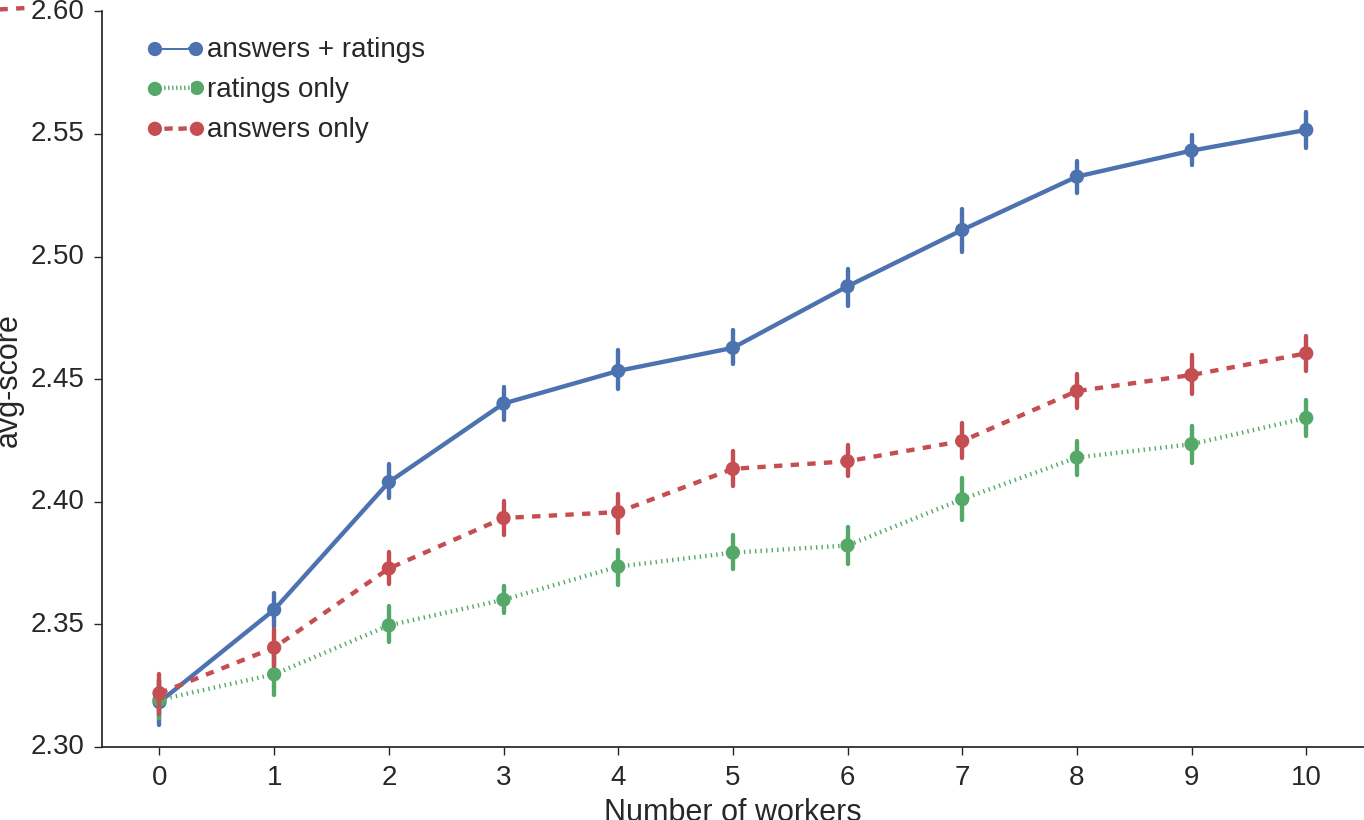
\includegraphics[width=\textwidth]{img/nworkers_vs_accuracy}
	\caption{avg-score: Average score per question}
	\label{fig:nworkers_vs_accuracy}
  \end{subfigure}
  \begin{subfigure}[t]{0.48\textwidth}
	\centering
	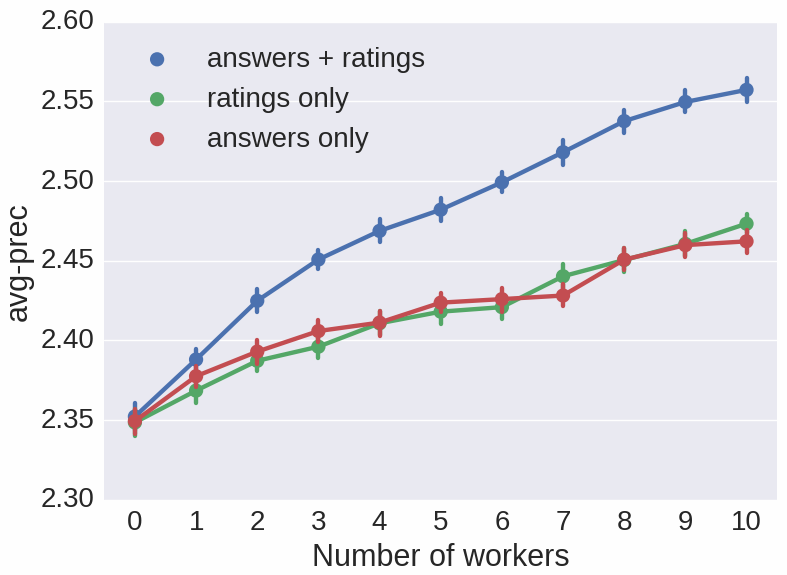
\includegraphics[width=\textwidth]{img/nworkers_vs_precision}
	\caption{avg-prec: Average score per answer (ignoring non-answered questions)}
	\label{fig:nworkers_vs_precision}
  \end{subfigure}
	\caption{Plot showing how the quality of the final answer depends on the number of workers per question}
	\label{fig:nworkers_vs_quality}
\end{figure*}

Obviously, more workers mean more reliable answer ratings and more answer candidates, which improves the performance of the question answering system.
However, we can observe diminishing returns, the cost per extra gain in performance metrics decreases as the number of workers grows.
Half of the overall performance improvements could be achieved with only 3 workers per question, which would save $\sim$70\% of the costs.

An alternative cost-reduction strategy is selective triggering of crowdsourcing, which would only ask for workers feedback for some of the questions.
Such a strategy would be necessary to scale a crowd-powered question answering system to a higher volume of questions.
There are multiple different approaches for such selective crowdsourcing: \eg a system can only ask for crowd contributions if it did not generate enough candidate answers or the predicted quality of the top scoring candidates was low~\cite{carmel2010estimating,he2006query}.
We leave these questions for the future work, as here we focused on the scenario, proposed by the organizers of the TREC LiveQA shared tasks, where questions arrive one by one and it is possible to utilize crowd input for every question.

To summarize, in the explored real-time QA scenario it is possible to reduce the costs of crowdsourcing by reducing the number of workers, although with some performance losses.
Our analysis suggests that paying $\sim$30\% of the original cost would give $\sim$50\% of the performance improvements.

\section{Related Work}
\label{sec:related_work}

Using the wisdom of a crowd to help users satisfy their information needs has been studied before in the literature.
For example, offline crowdsourcing can be used to prepare answers to tail search queries~\cite{bernstein2012direct}.
In this work, log mining techniques were used to identify potential question-answer pairs, which were then processed by the crowd to generate the final answer.
This offline procedure allows a search engine to increase the coverage of direct answers to user questions.
In our work, however, the focus is on online question answering, which requires fast responses to the user, who is unlikely to wait more than a minute.
Another related work is targeting a different domain, namely SQL queries.
The CrowdDB system of~\cite{franklin2011crowddb} is an SQL-like processing system for queries, that cannot be answered by machines only.
In CrowdDB human input is used to collect missing data, perform computationally difficult functions or matching against the query.
In~\cite{aydin2014crowdsourcing} authors explored efficient ways to combine human input for multiple choice questions from the ``Who wants to be a millionaire?'' TV show.
In this scenario going with the majority for complex questions is not effective, and certain answerer confidence weighting schemas can improve the results.  
CrowdSearcher platform of~\cite{Bozzon:2012:ASQ:2187836.2187971} proposes to use crowds as a data source in the search process, which connects a searcher with the information available through the users of multiple different social platforms.
In general, such websites open up many opportunities to interact with their users, in particular, identify users who might possess certain knowledge and request it by asking questions.
For example, \cite{nichols2012asking,nichols2013analyzing,mahmud2013recommending} showed that it is possible to get the information about airport security waiting times or product reviews by posting questions to a social network users, who identified themselves as being at an airport or mentioned the product of interest correspondingly.
While in this work, we primarily focused on more traditional way of hiring the crowd workers using Amazon Mechanical Turk, integration with social services is an interesting direction for the future work.

Many works have used crowdsourcing to get a valuable information that could guide an automatic system for some complex tasks.
For example, entity resolution system of \cite{Whang:2013:QSC:2536336.2536337} asks questions to crowd workers to improve the results accuracy.
Using crowdsourcing for relevance judgments has been studied extensively in the information retrieval community, \eg \cite{Alonso:2008:CRE:1480506.1480508,alonso2011design,grady2010crowdsourcing} to name a few.
The focus in these works is on document relevance, and the quality of judgments crowdsourced offline.
Whereas in our paper we are investigating the ability of a crowd to quickly assess the quality of the answers in a nearly real-time setting.
The use of crowdsourcing in IR is not limited to relevance judgments.
The work of \cite{harris2013comparing} explores crowdsourcing for query formulation task, which could also be used inside an IR-based question answering system.
\cite{lease2013crowdsourcing} provides a good overview of different applications of crowdsourcing in information retrieval.

Crowdsourcing is usually associated with offline data collection, which requires significant amount of time.
Its application to (near) real-time scenarios poses certain additional challenges.
\cite{bernstein2011crowds} introduced the retainer model for recruiting synchronous crowds for interactive real-time tasks and showed their effectiveness on the best single image and creative generation tasks.
VizWiz mobile application of \cite{bigham2010vizwiz} uses a similar strategy to quickly answer visual questions.
Our work builds on these ideas and uses the retainer model to integrate a crowd into a real-time question answering system.
The work of \cite{Lasecki:2013:CCC:2501988.2502057} showed how multiple workers can sit behind a conversational agent named Chorus.
Similarly to our work, Chorus used crowd workers to propose and vote on responses to user messages.
However, our CRQA system represents a hybrid approach to question answering, where the automatic QA module proposes certain answer candidates, and workers can judge their quality as well as propose additional responses.
Such an approach allows us to focus on more complex informational questions, for many of which the workers might not know the answer, but still can contribute by estimating the quality of automatically generated candidates.
Chorus, on the contrary, considered somewhat simpler tasks (\eg things to do in a new place, dinner date ideas, \etc), but focused more on maintaining a coherent dialog, which poses additional challenges, such as building a working dialog memory, keeping the users engaged with the dialog using gamification.
These ideas can be combined with the ideas of our work to build more intelligent assistants, that do not rely completely on the expertise of the workers.
Another use of a crowd for maintaining a dialog is presented in \cite{Bessho:2012:DSU:2392800.2392841}, who let the crowd handle difficult cases, when a system was not able to automatically retrieve a good response from the database of twitter data.

\section{Conclusions and Future Work} 
In this paper we presented CRQA, the first, as far as we know, real-time question answering system that integrated crowd work within an automatic QA system.
Specifically, we explore different methods of obtaining input from the crowd, and use a machine-learned answer re-ranking model that incorporates the crowd input as features to select the final system answer to return to the user. 

We report a large-scale experiment, in which over a thousand real user questions were submitted to the CRQA system in real time, as part of the LiveQA 2016 challenge.
CRQA was able to successfully answer these questions in under 1 minute, with over 80\% of the answers subsequently rated to be fair or better by human judges.
Importantly, CRQA significantly improved question quality and coverage compared to the starting automatic system, and, surprisingly, was often able to return a better answer, compared to the traditional CQA system with millions of users (Yahoo! Answers) with answers collected more than \textit{two days} after the original posting time.

The described CRQA implementation is a promising step towards efficient and close integration of crowd work and automatic analysis for real-time question answering.
It raises many promising issues and opens directions for future work, such as the performance of the crowdsourcing module when given less or more time to work, selective crowdsourcing for only the questions deemed ``difficult'' for the automatic system; more efficient online learning for obtaining ratings from the crowd and integrating them into the ranking model; and investigating additional features and sources of evidence for improving the joint ranking of the system and crowd input.
This paper provides a flexible and powerful framework for combining the powers of crowdsourcing with automatic question answering techniques, for building the next generation of real-time question answering systems.


\section{Acknowledgments}
The authors thank Scott Weitzner and Alec Wolyniec for helping with some experiments and contributing to the code used in system implementation.
The authors are also grateful to the anonymous reviewers for their valuable comments and suggestions.
This work was partially supported by the Yahoo Labs Faculty Research Engagement Program (FREP).

\bigskip
\bigskip

\bibliographystyle{aaai}
\bibliography{references}

\end{document}
